\chapter{O Orientado}

\begin{center}
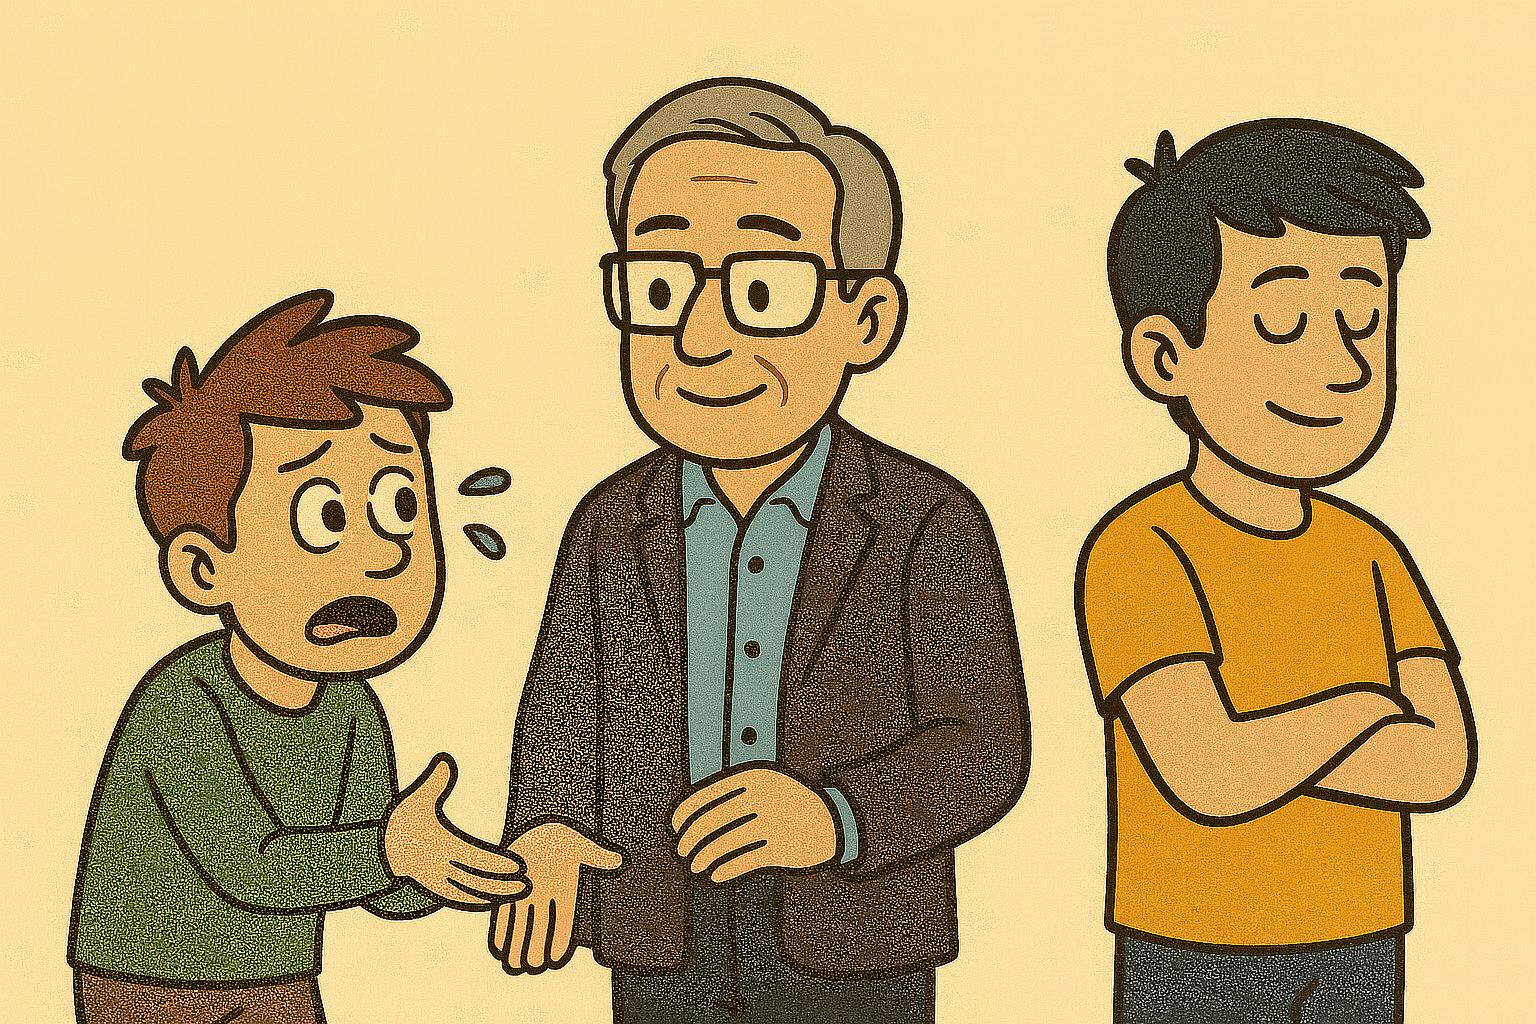
\includegraphics[width=0.5\linewidth]{Images/alunos.png}    
\end{center}
\vspace{0.5cm}

A tese é um projeto de uma só pessoa. Seu orientador, por mais interesse que tenha no assunto, não vai fazê-la por você. Isso seria, inclusive, antiético e ilegal.


A responsabilidade é basicamente sua e o sucesso será prioritariamente seu. Logo, a pessoa mais importante nesse projeto é você, pois é a única que pode completá-lo. Compreender a si mesmo é um fator importante nesse processo. Entender suas características, sejam elas positivas ou negativas, ajudará a alcançar seu objetivo.



\section{Conhecendo Suas Necessidades}

Antes de começar um projeto de mestrado ou doutorado, o aluno deve estar ciente de suas necessidades, limitações, restrições, capacidades e habilidades. Tudo isso deve ser levado em conta na sua preparação e mesmo na escolha se é o momento certo para realizar essa empreitada.

Em especial, quero chamar a atenção às necessidades. Um trabalho de extrema repercussão é o estudo de Maslow  sobre a hierarquia de necessidades das pessoas\footnote{Esse trabalho também foi muito criticado, mas certamente podemos utilizá-lo para exemplificar o fato de que você tem que estar bem em vários sentidos para ter a calma necessária para fazer sua tese.}. Ele é facilmente compreendido a partir da “pirâmide de Maslow”, que apresento na Figura \ref{fig:maslow}.

\begin{figure}
	\centering
	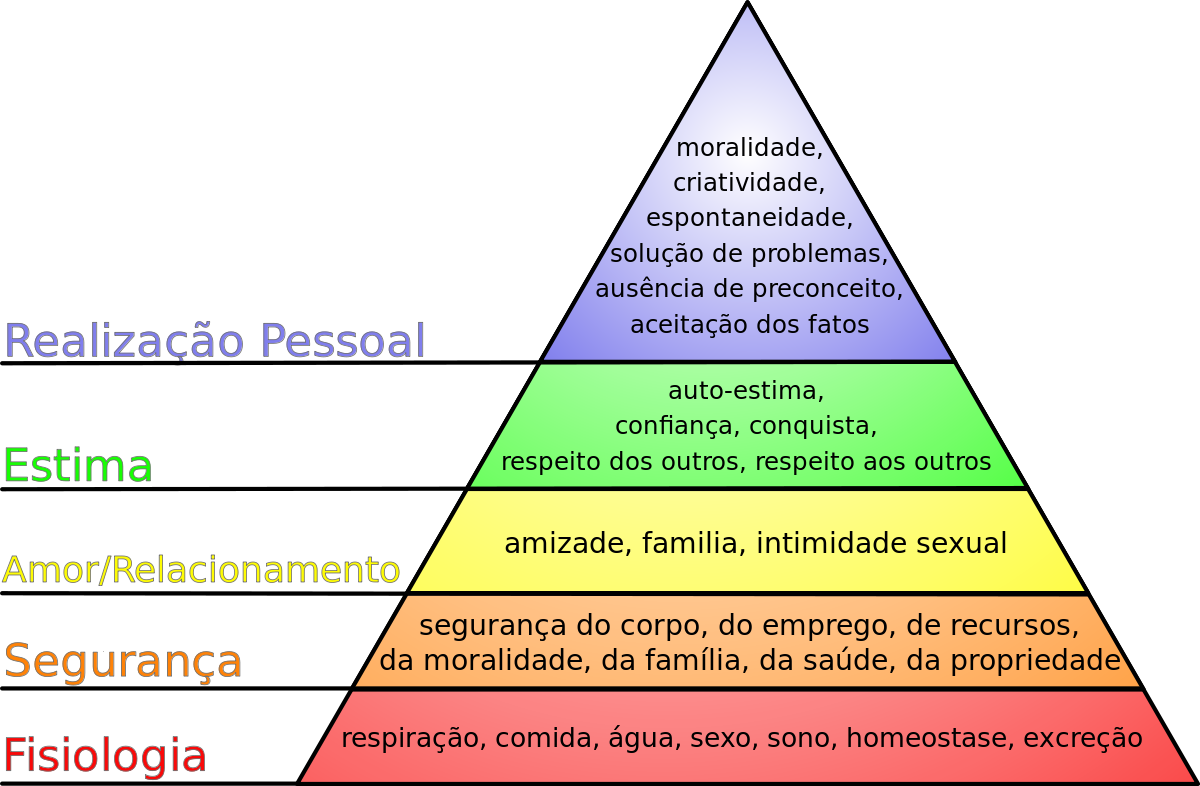
\includegraphics[width=0.7\linewidth]{Images/1200px-Hierarquia_das_necessidades_de_Maslow.svg}
	\caption{A pirâmide de Maslow.}
	\label{fig:maslow}
\end{figure}


Como se pode ver na Figura \ref{fig:maslow}, as necessidades são divididas em grupos e um grupo serve de base para todos os grupos superiores. Assim, as necessidades de realização pessoal (como fazer uma tese) são dependentes de todas as outras. 

Desse modo, podemos concluir que, para fazer uma pós-graduação, você deve garantir antes que tenha uma “boa base na pirâmide”. Isso significa garantir sua saúde, o modo de se manter, seus relacionamentos e sua autoestima.

Mesmo que você tenha começado sua dissertação ou tese em uma situação ideal, o longo prazo desse projeto, de 2 a 5 anos, implica em mudanças tanto no ambiente à sua volta quanto na sua própria vida. Alunos se casam, têm filhos, ficam doentes, se curam, precisam de mais dinheiro, se separam, trocam de emprego, tudo pode mudar nesse espaço de tempo.
Podemos citar como exemplo de acontecimento totalmente inesperado, e que afetou a todos em 2020/2021, a epidemia da Covid-19. Quantas vidas não foram mudadas? O impacto na vida dos mestrandos e graduandos foi muito variado e colocou um grande desafio para orientandos, orientadores e as instituições.

Voltando a pirâmide, ela indica que qualquer problema em uma camada inferior afeta diretamente a camada superior. Você deve estar consciente dessa estrutura e saber que problemas de qualquer tipo sempre afetarão seu rendimento na camada do topo, seja ocupando seu tempo, seja ocupando sua mente. Cabe ao aluno perceber e controlar o grau desse efeito e, quando necessário, interagir com o orientador.

Por isso não hesite em procurar seu orientador e avisá-lo do que está acontecendo com você. Mesmo que ele não possa ajudá-lo no problema específico, ele compreenderá e tentará ajudar no que for possível. 
Exemplos típicos de coisas que acontecem na vida de um aluno: um novo emprego ou uma situação de desemprego, troca de chefes que afeta a liberação ou o interesse da empresa, doenças mais ou menos graves consigo ou com parentes, perda de acesso aos dados prometidos por alguém, gravidez, casamento, etc.

O orientador não é um sargento empurrando você em uma marcha forçada. Ao contrário, ele é o guia que evita que você se perca em uma exploração. 
Ele está ali para auxiliá-lo nos percalços do caminho, até mesmo para dizer que está na hora de parar e tentar em outra expedição. 
Uma relação de boa qualidade com o orientador é uma das mensagens que quero passar nesse texto. Ela vai facilitar sua vida e chegar ao seu objetivo.

\section{A Saúde Mental do Aluno}

Realizar uma dissertação ou tese é um processo longo, exigente e, por vezes, solitário. Não é incomum que alunos passem por períodos de ansiedade, estresse, desmotivação ou mesmo depressão ao longo dessa jornada. A intensidade do trabalho intelectual, a pressão por produtividade, os prazos e as incertezas sobre o futuro são fatores que, somados, podem afetar negativamente a saúde mental.

Infelizmente, ainda há certo tabu na academia sobre reconhecer que estamos sobrecarregados emocionalmente. Muitos alunos sentem que precisam manter uma aparência de resiliência constante, o que apenas agrava o sofrimento. A saúde mental, contudo, não é um luxo ou um detalhe — é um requisito fundamental para o bom andamento da pesquisa.

\gxatencao{Ninguém consegue escrever bem, propor soluções criativas ou analisar dados com clareza se está exausto, ansioso ou emocionalmente abalado.}

Por isso, é fundamental que você preste atenção aos sinais de alerta:
\begin{itemize}
    \item Dificuldade prolongada de concentração ou produtividade;
    \item Sensação de culpa constante por “não fazer o suficiente”;
    \item Sentimento de isolamento ou de incapacidade;
    \item Episódios de ansiedade, insônia ou crises de choro frequentes;
    \item Desinteresse persistente pelas atividades que antes eram prazerosas;
    \item Pensamentos negativos recorrentes.
\end{itemize}

Se perceber algum desses sinais, não os ignore. Procure ajuda profissional, como psicólogos e psiquiatras. Muitas universidades oferecem gratuitamente apoio psicológico aos alunos. Grupos de apoio, colegas de confiança e familiares também podem ser fontes importantes de acolhimento.

Além disso, mantenha práticas saudáveis no dia a dia:
\begin{itemize}
    \item Durma bem e mantenha uma rotina regular;
    \item Alimente-se adequadamente;
    \item Reserve tempo para atividades físicas e lazer;
    \item Estabeleça limites entre o tempo de estudo e o tempo pessoal;
    \item Evite o perfeccionismo excessivo — ele é um sabotador frequente.
\end{itemize}

Em momentos de sobrecarga emocional, seu orientador pode ajudá-lo a ajustar metas, redefinir prazos ou até mesmo propor uma pausa estratégica. Ocultar seu estado emocional pode apenas agravar a situação e comprometer o projeto como um todo.

\gxatencao{Cuidar da saúde mental não é sinal de fraqueza — é demonstração de maturidade, responsabilidade e inteligência emocional.}

Lembre-se: a pós-graduação é um projeto importante, mas sua vida e seu bem-estar vêm antes. 

\CoppeWay{O Serviço Acolhe Coppe}{

O \textbf{Acolhe Coppe} oferece atendimento individual breve, rodas de conversa, grupos temáticos, encontros de arteterapia, acolhimento para aposentadoria, entre outras atividades. 
Seus objetivos incluem proporcionar escuta qualificada, ampliar direitos, fortalecer vínculos e oferecer suporte para que os indivíduos enfrentem as dificuldades vividas ao longo da vida acadêmica e profissional. 
Ressalta-se que o Acolhe Coppe \textbf{não substitui} o acompanhamento clínico-psicológico oferecido pelo SUS ou redes particulares, mas atua de forma complementar.

\gxatencao{Todo aluno da Coppe pode buscar apoio no Acolhe Coppe de forma gratuita, com sigilo e respeito à individualidade.}

O acesso ao serviço é simples e pode ser feito pelos seguintes canais:

\begin{itemize}
    \item \textbf{Site oficial:} \href{https://acolhecoppe.dgesp.coppe.ufrj.br}{https://acolhecoppe.dgesp.coppe.ufrj.br}
    \item \textbf{E-mail institucional:} \href{mailto:acolhecoppe@adc.coppe.ufrj.br}{acolhecoppe@adc.coppe.ufrj.br}
    \item \textbf{Localização:} Centro de Tecnologia (CT), Bloco H, Sala 121B – Ilha do Fundão – UFRJ
\end{itemize}
}

\section{Os Estereótipos}

Uma maneira de compreender a si mesmo é conhecer estereótipos comuns das pessoas e ver até que ponto você se encaixa nesses estereótipos. 


Existem muitos tipos de alunos. Um orientador, com o tempo, desenvolve sua fórmula pessoal para tratar cada um deles. No texto a seguir, apresentarei alguns estereótipos. Raramente um aluno segue fielmente um desses estereótipos, mas eles servem como referência.


 Fique certo que muitos irão avaliar seu desempenho, principalmente seus orientadores. 
 Muitas vezes receberá críticas, algumas justas, outras não. 
 Entender a si mesmo e entender por que as pessoas o percebem de certa forma o ajudará a progredir.


Os alunos têm diferentes graus de dependência, ou independência, do orientador. A maioria dos alunos passa, durante a tese, por vários desses “graus”. Vamos analisar como funcionam os alunos estereotipados: o totalmente dependente e os totalmente independentes.


\subsection{O estereótipo independente}


O aluno totalmente independente é normalmente uma pessoa com interesses bem específicos. Escolhe um tema que o orientador pode auxiliar, mas não é necessariamente especialista. Sua relação de orientação é feita a partir da comunicação de tempos em tempos, ao orientador, do que está fazendo. Nessa conversa, tem sempre uma proposta de solução quando apresenta um problema e procura conhecer a opinião do orientador. 


Tive bons alunos desse tipo. Talvez todos eles tenham se envolvido, em alguma parte da tese, em problemas.


Um dos problemas que podem acontecer é que esse aluno, por se manter distante do orientador, tanto fisicamente quanto em relação ao tema de tese, não consiga imprimir um ritmo adequado sozinho. Isso se torna mais crítico quando o aluno tem alguma dificuldade pessoal grave e acaba “sem tempo” de informar o orientador.


\gxatencao{O aluno deve informar imediatamente ao orientador de qualquer problema pessoal que esteja dificultando ou impedindo seu progresso.
}

Principalmente com problemas emocionais, de saúde e financeiros graves, com si mesmo ou com sua família, o aluno deve informar o orientador e tomar com ele decisões como continuar trabalhando, ou suspender o trabalho ou até mesmo, e muito raramente, abandonar a tese. 

\gxatencao{O importante é que o aluno traga o problema ao orientador antes de criar um problema com seu prazo ou com suas avaliações}.


Outra coisa que pode acontecer é o aluno independente achar que o orientador o abandonou. Ele nunca fala com o orientador e, nas raras vezes que fala ou tenta falar, o orientador está muito ocupado. O orientador pode achar que o aluno o abandonou também, já que o aluno nunca o procura. Na verdade, pode ser que ambos tenham razão. 


Se houver alguma comunicação entre os dois e essa comunicação for clara, e a iniciativa do aluno for boa, a tese deve ser concluída. Se o aluno perder a iniciativa, o orientador terá trabalho para recolocá-lo nos trilhos, talvez não consiga. Se a comunicação for pequena o aluno corre o risco de querer fazer coisas demais e não acabar a tese ou fazer tudo errado, pois não sabe algum detalhe importante que o orientador já estudou.


No limite, alguns alunos desprezam a orientação, acham que o orientador não sabe o que está fazendo, ou simplesmente não ligam para a orientação.


Isso é péssimo. O orientador é mais experiente que o aluno e, se não tem a percepção localizada do assunto, por estar estudando menos o tema que o aluno naquele instante, tem a percepção generalizada bem mais apurada que a do aluno. Por isso que um é orientador e o outro aluno.


Um ditado típico da minha família é:


\gxatencao{O diabo não é perigoso por ser mais inteligente. 
O diabo não é perigoso por ser mais forte. 
O diabo é perigoso porque é mais velho.}


O orientador é mais velho, ou pelo menos está há mais tempo na área. Ou seja, o aluno independente tem muitas características boas, porém tem um risco muito alto.


\subsection{O estereótipo dependente}


Do outro lado do espectro, existe o aluno totalmente dependente. Esse aluno não faz nada sem perguntar ao orientador. Não tem ideias próprias. Desenvolve trabalhos a partir da orientação do orientador e fazendo implementações segundo algoritmos definidos pelo orientador. Nunca perde o contato. 


Supondo que esse aluno é competente, ele é um aluno de risco baixo. Tem grandes chances de acabar a tese, porque faz tudo que o orientador manda e o orientador deve saber em que direção vai à tese. 


Os riscos em relação a esse aluno ocorrem se orientador estiver em uma fase muito criativa, mas sem foco ou sem tempo. 


Outro risco importante é o aluno não se identificar com a tese, porque foi escolhida pelo orientador. 


\subsection{O aluno real}


Se você olhar as descrições acima com cuidado vai perceber algo estranho: o aluno independente, supostamente o melhor aluno, é o que corre mais riscos. Isso acontece porque tanto a construção de uma dissertação ou tese quanto a orientação são processos. Quanto mais o orientado faz parte do processo, mais chances têm que terminá-lo de forma satisfatória.


Obviamente, nenhum aluno é totalmente independente ou dependente. Pessoalmente, tive boas relações com alunos em vários pontos do espectro. O importante é que o aluno permaneça em contato com o orientador. 


Aviso aos orientados que é o aluno que se mantém em contato com o orientador, não o inverso. É o aluno que deve procurar, marcar reuniões, trazer o trabalho. É o orientado que deve esperar pelo orientador na porta de sua sala. O orientador possui vários alunos e tarefas, dificilmente consegue controlar a frequência de cada um. Lembre-se, você é um dos alunos de seu orientador, enquanto seu orientador é o único que você tem.


\gxatencao{O aluno deve se manter em contato com o orientador.}


Uma história pessoal: quando queria falar com meu orientador sozinho, sem interrupção, eu pegava uma carona. Era a única forma de ter um “tempo só para mim”. E nem sempre dava certo.


\subsection{Como se avaliar quanto à independência}


Tente responder as seguintes perguntas:
\begin{itemize}
	\item Eu converso com meu orientador com uma frequência fixa?
	\item Quantas vezes por mês eu converso com meu orientador?
	\item Meu orientador é capaz de dizer em que ponto eu estou na minha tese?
	\item Meu orientador é capaz de falar sobre minha tese?
\end{itemize}



